\section{Results}

\subsection{Traits and diversification}

% E: I brutally shortened the text here and hence put all the models into one section for the "diversification" question.  But I think I retained all the ideas that were written out before.
% Much of what I removed was descriptions about which distributions are/aren't overlapping with one another.  I think that's easier for the reader to see in the figures than to read in the text.  But now the text says things like if some estimates are "different", so perhaps in Methods we should explain different = non-overlapping?
% For the former model comparison section, I moved the key conclusions into the paragraphs here and the mechanical details (bayes factor definition) into Methods.

We found that when considered alone, ploidy and breeding system each showed significant associations with net diversification differences. %B: check and deleteme: I think this should have "states" added, so "...ploidy and breeding system states showed..."
When considered together, however, the effect of breeding system dominated the effect of ploidy, although hidden factors played an important role as well. %B: same here.

%B: The "For X (states model), we found" template doesn't sound quite right to me. Maybe, "Fitting" or "Considering" or "When" (as in second portion with hidden-state model. In latter case, possibly (1) When considering X alone..., (2) Addition of... / Incorporating a hidden state...
%
For ploidy alone (D/P model), we found a greater net diversification rate for diploids than for polyploids, in agreement with \citep{mayrose_2011, mayrose_2015}.
This result holds with (\cref{figure:netdivall}A) or without (\cref{figure:netdivnodip}A) the diploidization parameter, though including diploidization shifts the net diversification rate of polyploids to be non-negative.
Incorporating a hidden state, however, removes the clear separation in diversification between diploids and polyploids (D/P+A/B model; \cref{figure:netdivall}B, \cref{figure:netdivnodip}B).
Thus, differences in net diversification are better explained by an unknown factor than by ploidy.
Statistical model comparisons show very strong support for including the hidden state and strong support for including diploidization (\cref{table:bayesfactors}).
% E: I removed the description of relative extinction results.  We don't discuss it for other models or show it in the main text, and I never really know what to make of that compound parameter.  But it's good that it's in the supp info.

For breeding system alone, we found a larger net diversification rate for SI than for SC species, in agreement with \citet{goldberg_2010} (I/C model, \cref{figure:netdivall}C).
When a hidden state is included (I/C+A/B model), the large net diversification difference persists for one of the hidden states but is removed for the other (\cref{figure:netdivall}D).
Thus, differences in net diversification are best explained by both breeding system and an unknown factor.
% The transition rate from SI to SC is $q_{IC}=0.3$ for both the I/C and the I/C+A/B models.
The statistical model comparison shows very strong support for including the hidden state (\cref{table:bayesfactors}).

For ploidy and breeding system together (ID/CD/CP model), the net diversification rate for SI diploids was greater than for either SC diploids or SC polyploids, with or without diploidization (\cref{figure:netdivall}E, \cref{figure:netdivnodip}C).
It thus appears that the difference in net diversification with breeding system persists when ploidy is included in the model, but not the reverse.
The association of ploidy with net diversification in the D/P model (\cref{figure:netdivall}A, \cref{figure:netdivnodip}A) appears to be driven by the subset of diploids that are SI; among SC species, net diversification rates for diploids and polyploids are similar.
%
When a hidden state is included (IC/CD/CP+A/B model), the same general pattern remains when diploidization is prevented (\cref{figure:netdivnodip}D), although the higher net diversification rate of ID is less clear within one of the hidden states.
With diploidization, the net diversification rate of ID is still greater than CD within each hidden state, but diversification for P is highly uncertain and perhaps bimodal.
Statistical model comparisons show very strong support for including the hidden state and at most positive support for including diploidization (\cref{table:bayesfactors}).

% E: I moved the discussion of \rho_I and \rho_C values into the Pathways section.
% E note to self: keep editing from here XXX

\subsection{Diploidization as an exploratory hypothesis}

For the two models that only consider diploid and polyploid state (D/P and D/P+A/B) the effect of removing parameter $\delta$ was that net diversification rate of polyploids can be negative with high probability (\cref{figure:netdivnodip}AB).
However, in the models that simultaneously considered polyploidy and breeding system, removing the $\delta$ parameter did not have much of an effect on the location of the posterior distribution of polyploid net diversification rate but on the credible interval width and overlap with net diversification of diploids.
When diploidization was absent, the net diversification of polyploids overlaps with the net diversification of self-compatible diploids but not with the one of self-incompatible diploids (\cref{figure:netdivnodip}CD).
For all models, the posterior distribution of diploidization rate is more uncertain than the one of polyploidization rates (see supplementary information figures). 

\subsection{Pathways to polyploidy}

% E: If we're going to include pathway results for real, I need to write more in this section and incorporate the figure.  TODO

Polyploidization rates from self-compatible diploid $\rho_{CD}$ and from self-incompatible diploid $\rho_{ID}$ are not significantly different (see supplementary information figures).
However, the distribution of $\rho_{ID}$ seems to always consider faster values compare to the distribution of $\rho_{CD}$.
This result is highlighted in ancestral reconstructions of the $ID/CD/CP$ model where transitions from ID to CP are more probable than transitions from CD to CP. % Emma here we put the figure?


\begin{supptable}
    \begin{center}
    \begin{tabular}{lcccccc}
                       & D/P   & D/P+A/B      & I/C    & I/C+A/B      & ID/CD/CP & ID/CD/CP+A/B \\ \midrule
        %                                                                                      
        $r_D$          & 0.382 & 0.698, 0.100 & ---    & ---          & ---      & ---          \\
        $r_P$          & 0.109 & 0.587, 0.182 & ---    & ---          & ---      & ---          \\
        $r_I$          & ---   & ---          & 0.550  & 0.386, 0.877 & ---      & ---          \\
        $r_C$          & ---   & ---          &-0.001  &-0.059, 0.606 & ---      & ---          \\
        $r_{ID}$       & ---   & ---          & ---    & ---          & 0.449    & 0.318, 0.789 \\
        $r_{CD}$       & ---   & ---          & ---    & ---          & 0.050    &-0.248, 0.494 \\
        $r_{CP}$       & ---   & ---          & ---    & ---          &-0.027    & 0.110, 0.634 \\
        %                                                                                      
        $\rho$         & 0.033 & 0.026        & ---    & ---          & ---      & ---          \\
        $\rho_I$       & ---   & ---          & ---    & ---          & 0.063    & 0.047        \\
        $\rho_C$       & ---   & ---          & ---    & ---          & 0.024    & 0.011        \\
        $\delta$       & 0.050 & 0.162        & ---    & ---          & 0.022    & 0.107        \\
        $q_{IC}$       & ---   & ---          & 0.364  &              & 0.194    & 0.164        
    \end{tabular}

    \vspace{12pt}
    \begin{tabular}{lcccc}
                       & D/P   & D/P+A/B      & ID/CD/CP & ID/CD/CP+A/B \\ \midrule
        %                                                              
        $r_D$          & 0.260 & 0.193, 0.658 & ---      & ---          \\
        $r_P$          &-0.056 & 0.030, 0.187 & ---      & ---          \\
        $r_I$          & ---   & ---          & ---      & ---          \\
        $r_C$          & ---   & ---          & ---      & ---          \\
        $r_{ID}$       & ---   & ---          & 0.455    & 0.309, 0.797 \\
        $r_{CD}$       & ---   & ---          & 0.065    &-0.006, 0.587 \\
        $r_{CP}$       & ---   & ---          &-0.088    &-0.074, 0.403 \\
        %                                                              
        $\rho$         & 0.047 & 0.047        & ---      & ---          \\
        $\rho_I$       & ---   & ---          & 0.067    & 0.053        \\
        $\rho_C$       & ---   & ---          & 0.033    & 0.032        \\
        $q_{IC}$       & ---   & ---          & 0.198    & 0.145        
    \end{tabular}
    \end{center}
    \caption{
        Median rate estimates for all models.
        Units are per million years.
        Two comma-separated numbers refer to the $A$ and $B$ hidden states, and --- means the parameter was not present in the model.
        The upper section is for models with diploidization, and the lower section is for models without.
        The supplemental figures show the corresponding distributions of parameter estimates.
    }
    \label{table:estimates}
\end{supptable}

\begin{figure}
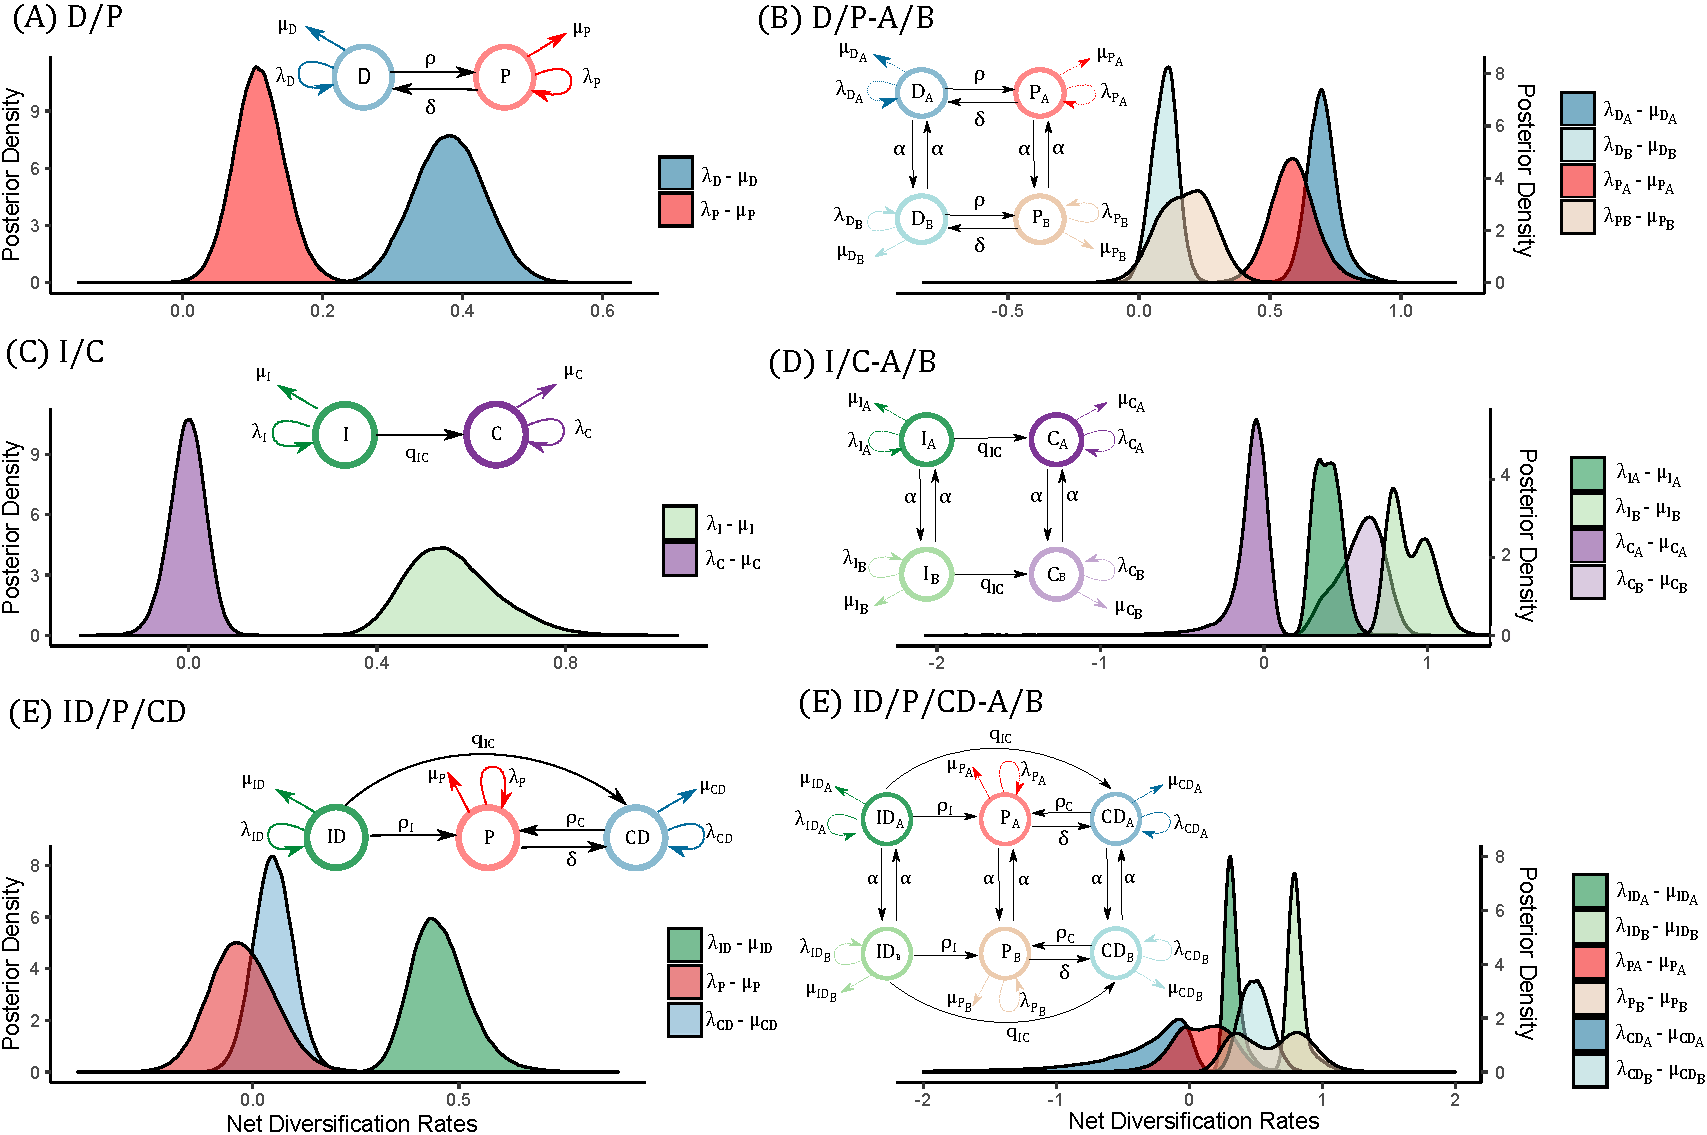
\includegraphics[width=\textwidth]{Netdiversificationallmodels.pdf} % FIXME: The panel labels should use "+A/B" instead of "-A/B".  Rosana, if you add the .svg file for this figure, I can make small changes like this.
\caption{Net diversification rates for all models that include diploidization.}  
\label{figure:netdivall}
\end{figure}

\begin{figure}
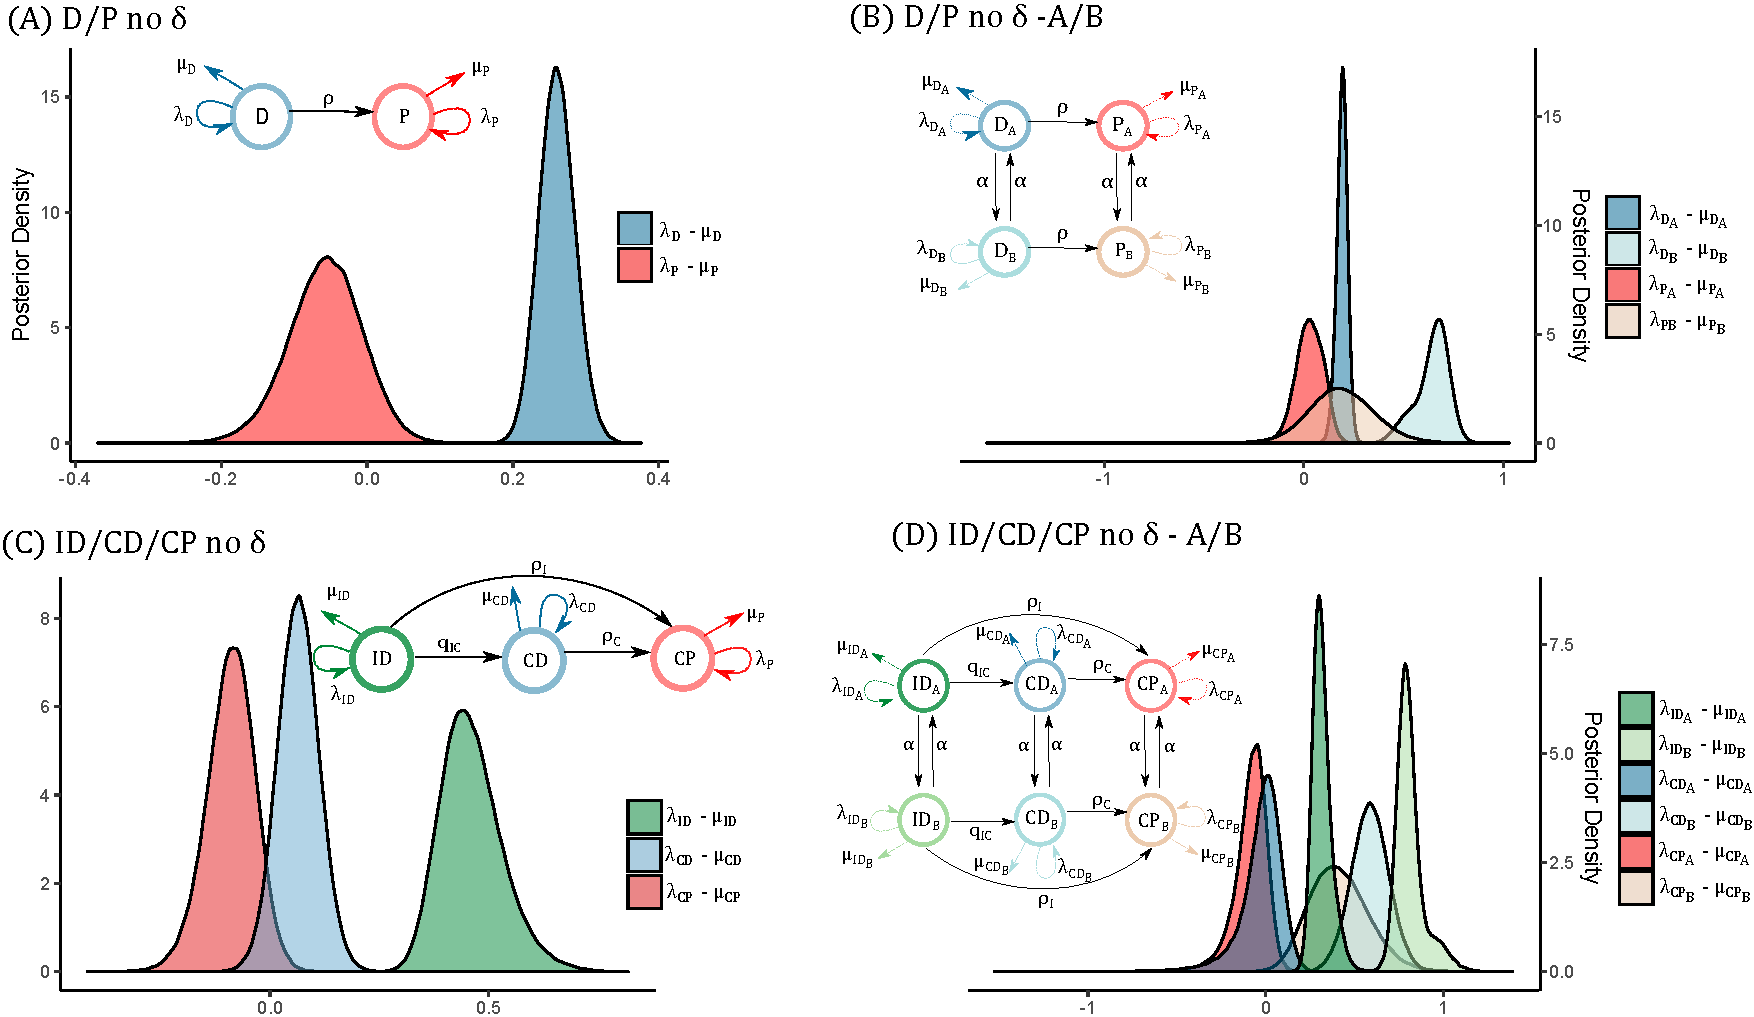
\includegraphics[width=\textwidth]{netdiversificationallnodip.pdf} % FIXME: same note as above about "+A/B"
\caption{Net diversification rates for all models that do not include diploidization.}  
\label{figure:netdivnodip}
\end{figure}

\begin{suppfigure}
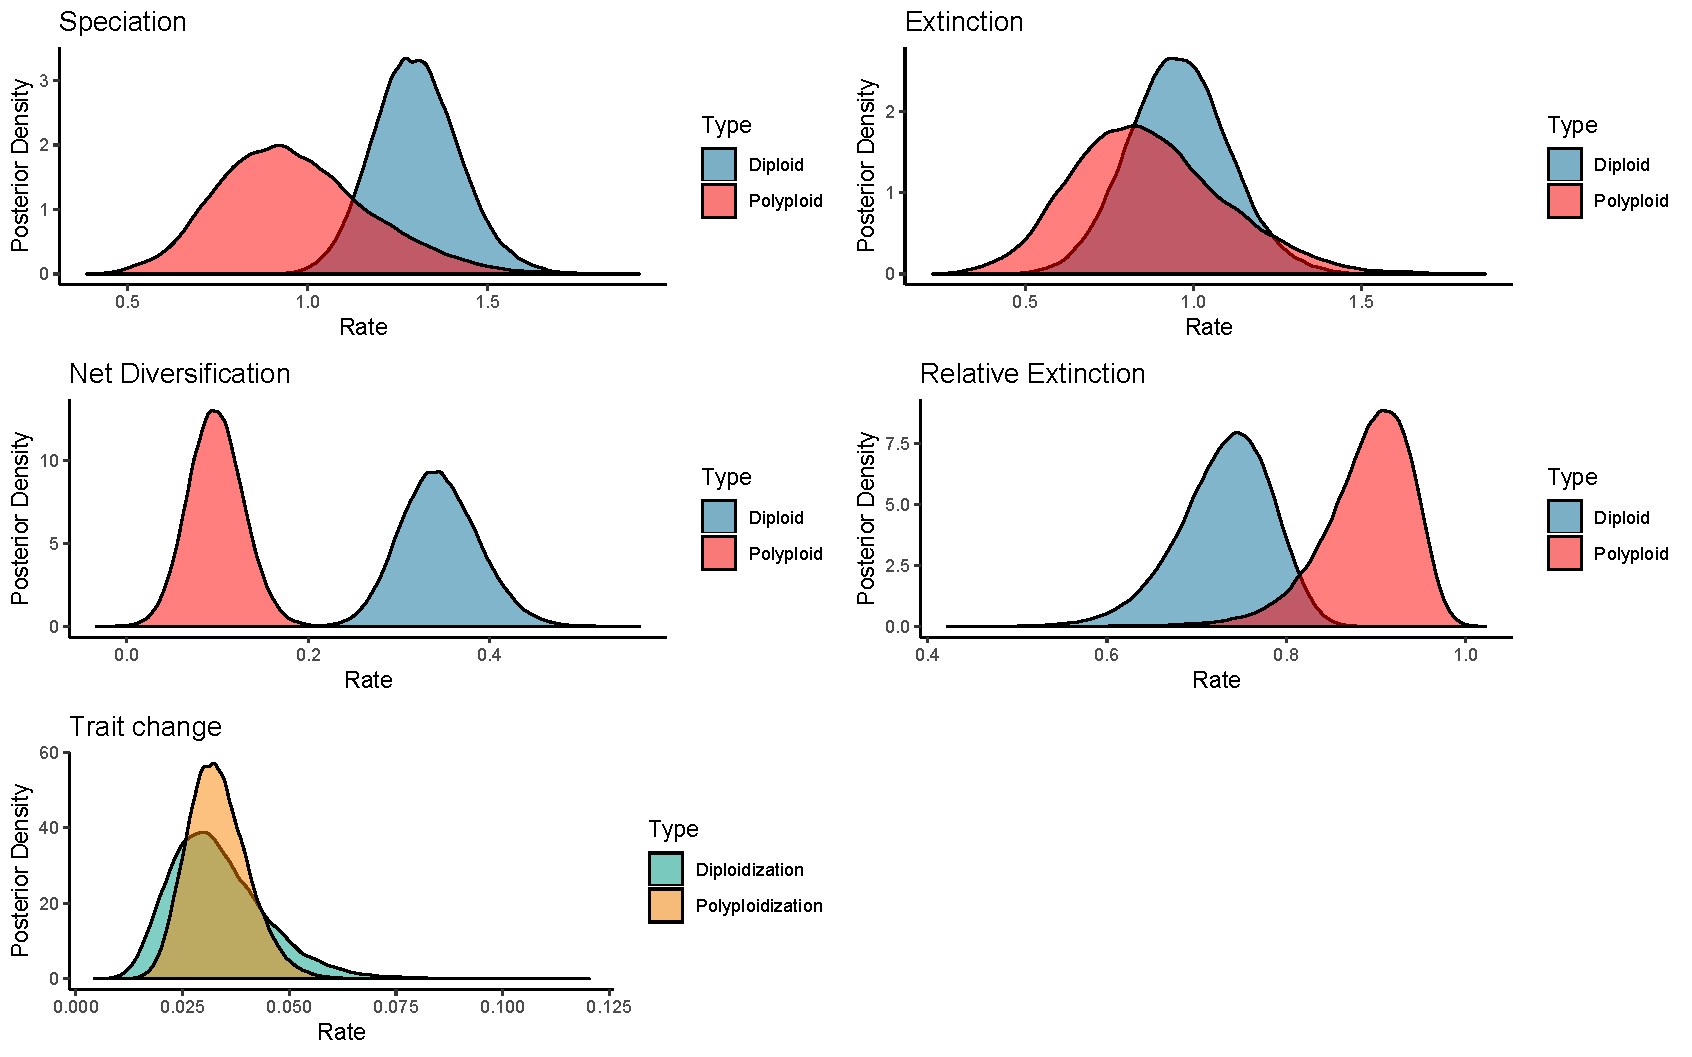
\includegraphics[width=\textwidth]{bisseDPposteriordist.pdf}
\caption{Posterior distribution for each of the parameters in the D/P polyploidy model} % XXX
\label{suppfigure:DP}
\end{suppfigure}

\begin{suppfigure}
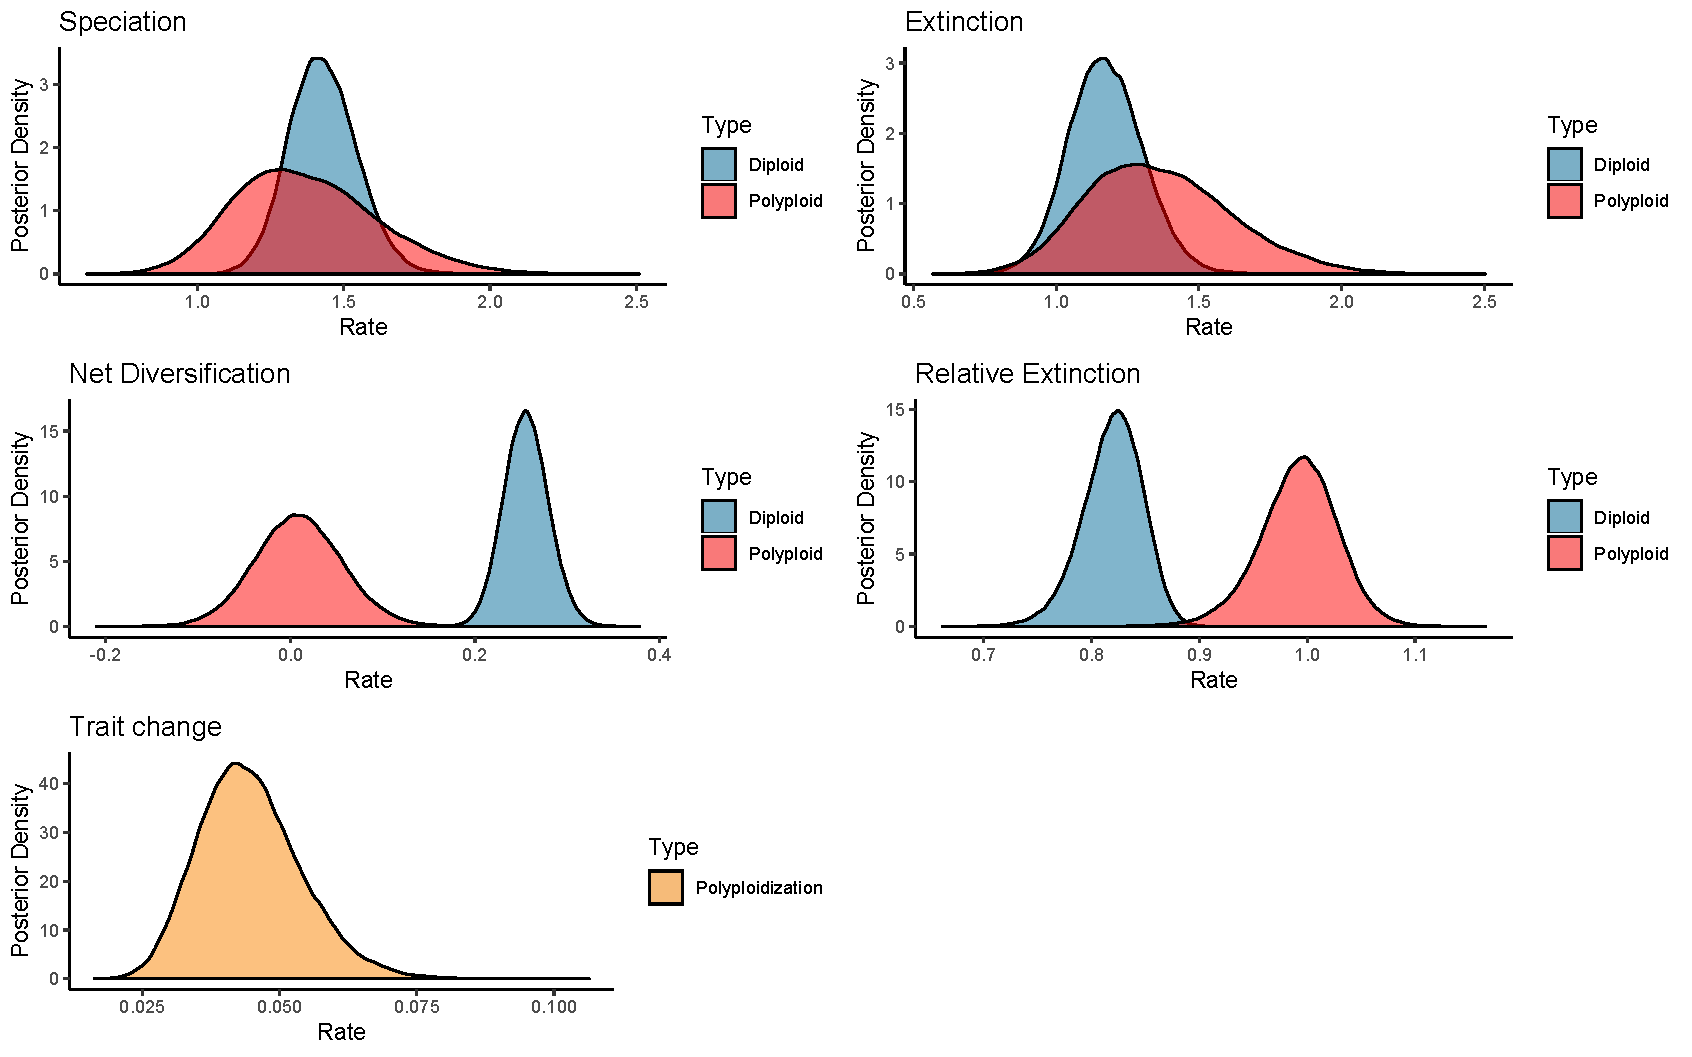
\includegraphics[width=\textwidth]{bisseDPnodipposteriordist.pdf}
\caption{Posterior distribution for each of the parameters in the D/P no $\delta$ polyploidy model} % XXX
\label{suppfigure:DPnodip}
\end{suppfigure}

\begin{suppfigure}
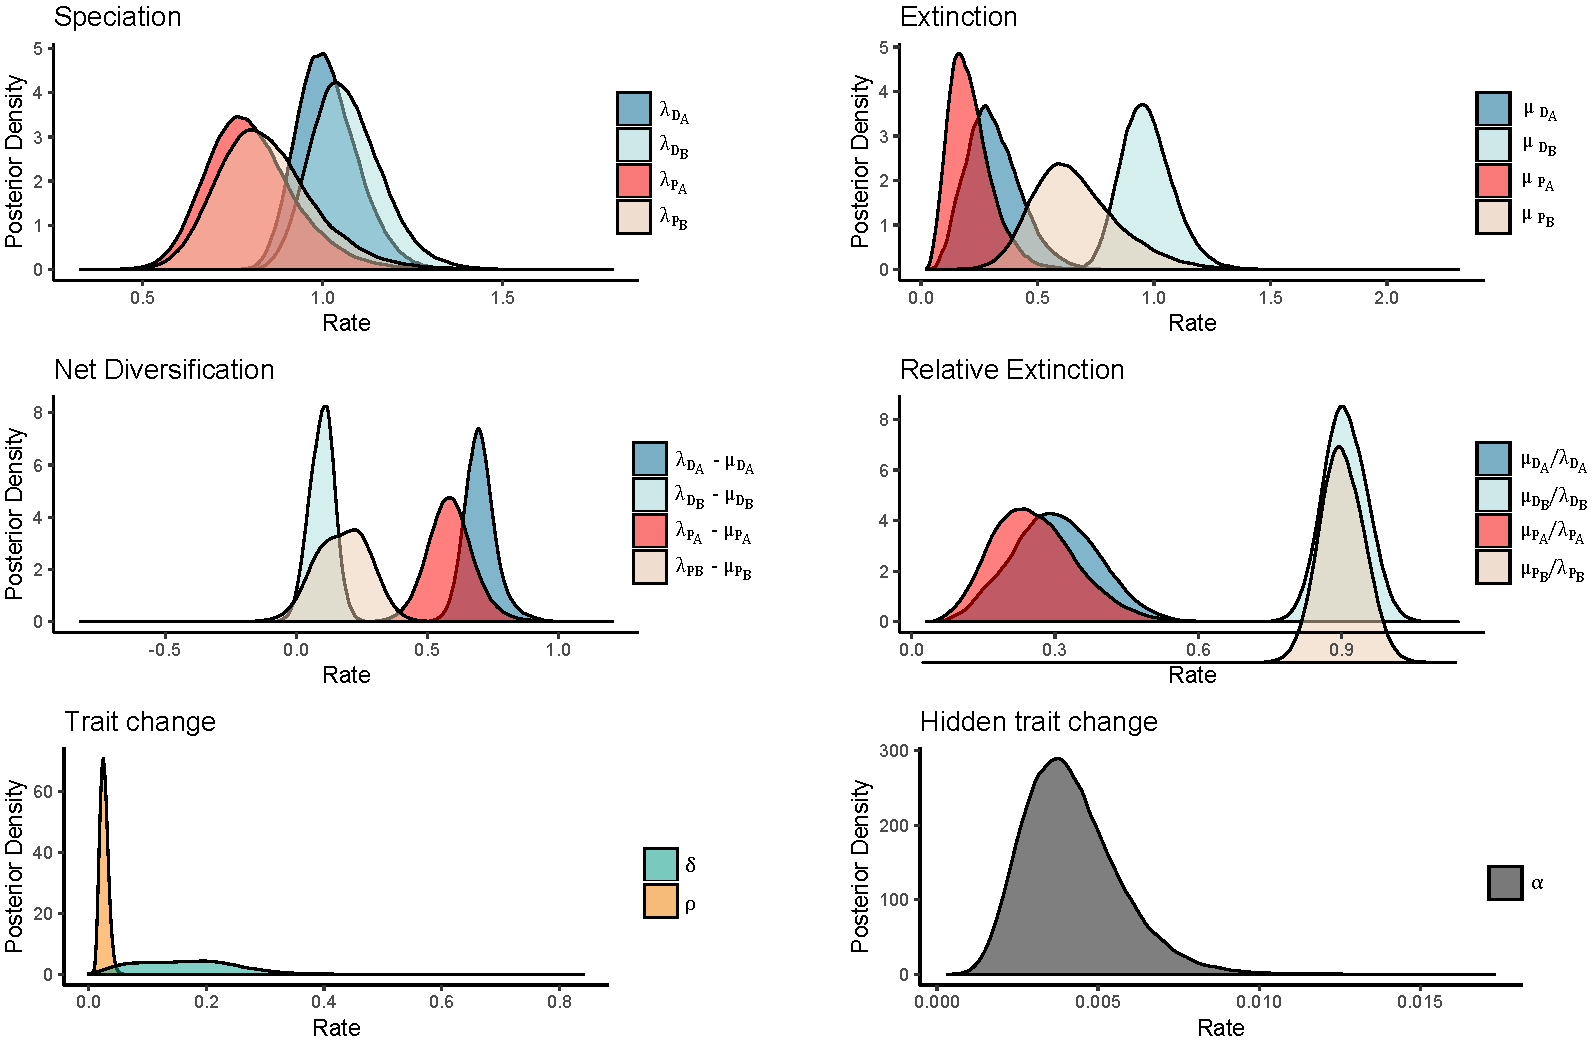
\includegraphics[width=\textwidth]{hisseDPposteriordist.pdf}
\caption{Posterior distribution for each of the parameters in the D/P-A/B polyploidy model} % XXX
% fixme: offset plotting error in "relative extinction" panel
\label{suppfigure:DPAB}
\end{suppfigure}

\begin{suppfigure}
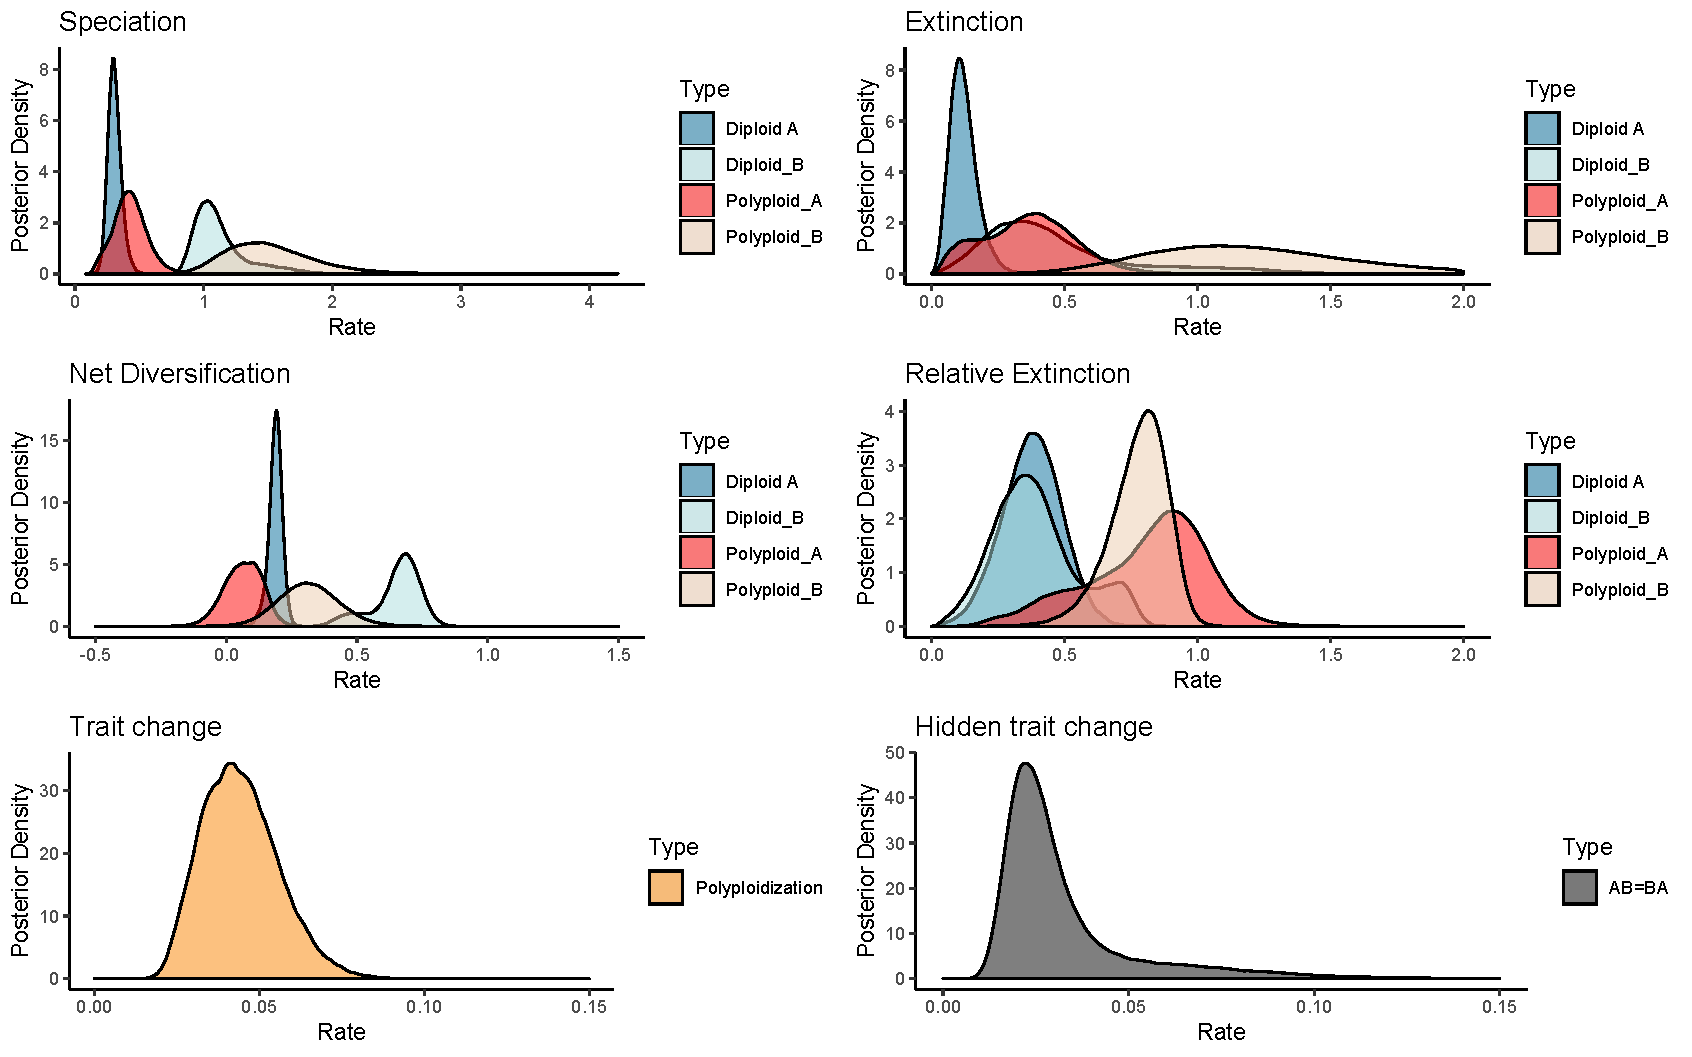
\includegraphics[width=\textwidth]{hisseDPnodipposteriordist.pdf}
\caption{Posterior distribution for each of the parameters in the D/P no $\delta$-A/B polyploidy model} % XXX
\label{suppfigure:DPnodipAB}
\end{suppfigure}

\begin{suppfigure}
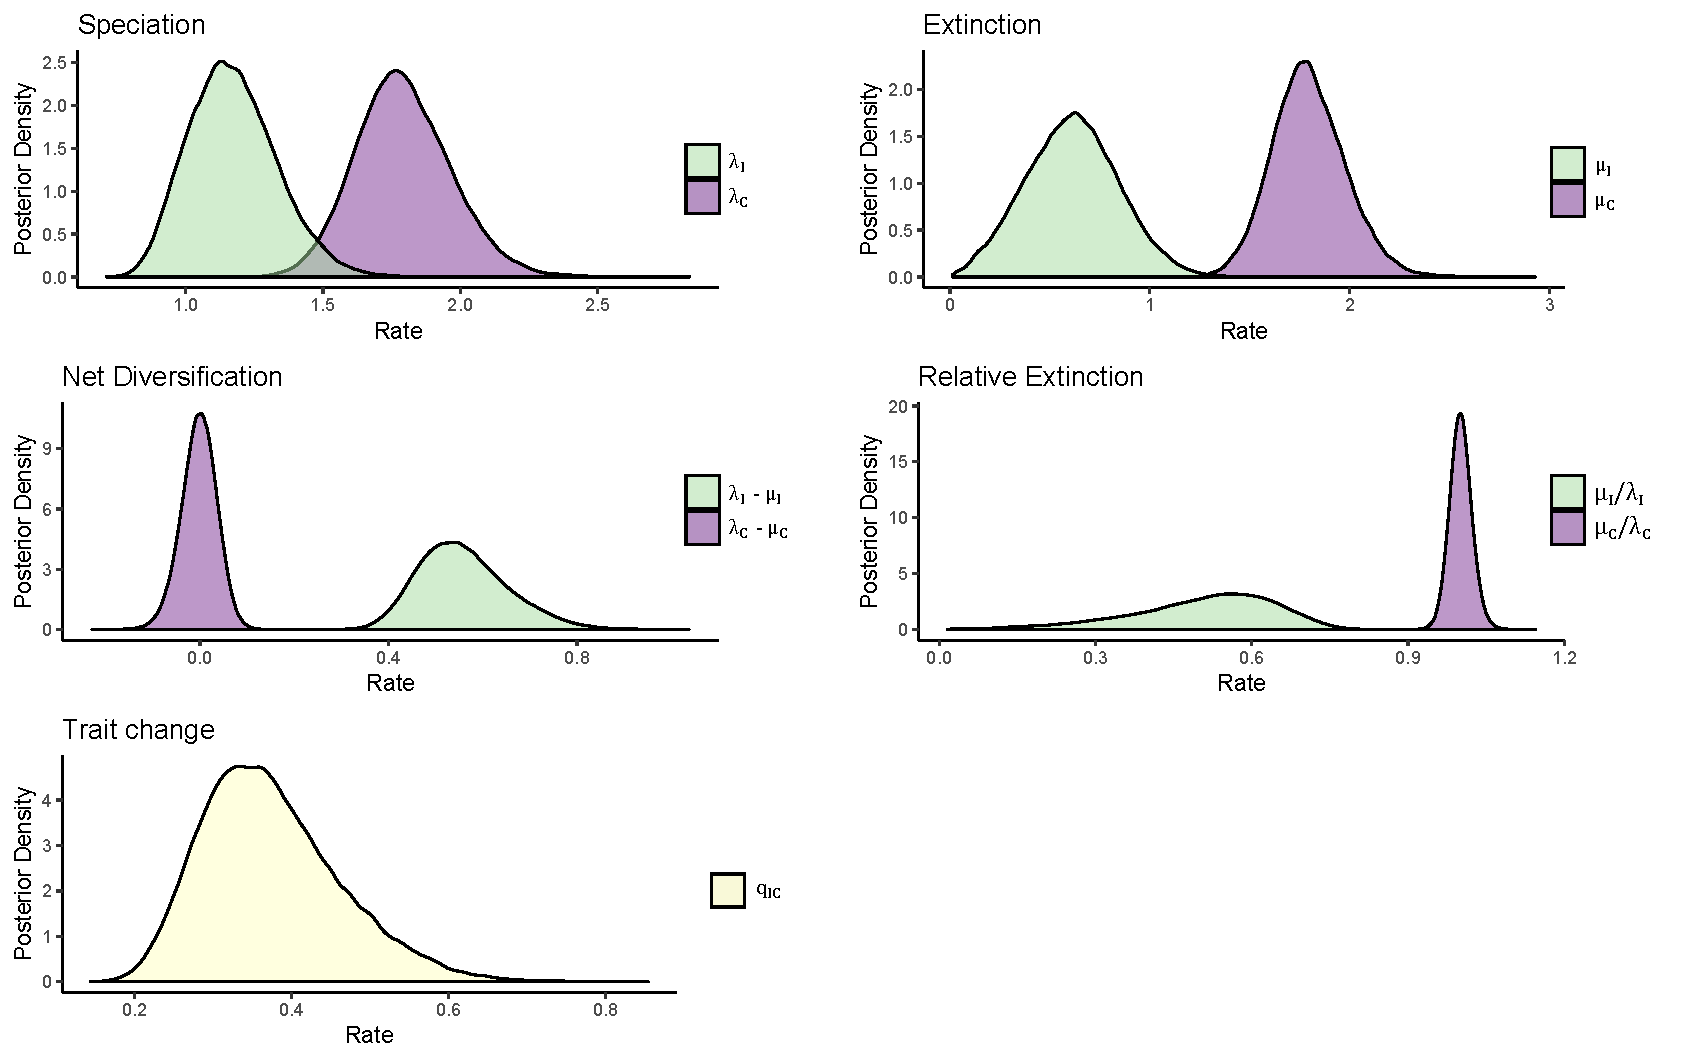
\includegraphics[width=\textwidth]{bisseSIposteriordist.pdf}
\caption{Posterior distribution for each of the parameters in the I/C breeding system model} % XXX
\label{suppfigure:IC}
\end{suppfigure}

\begin{suppfigure}
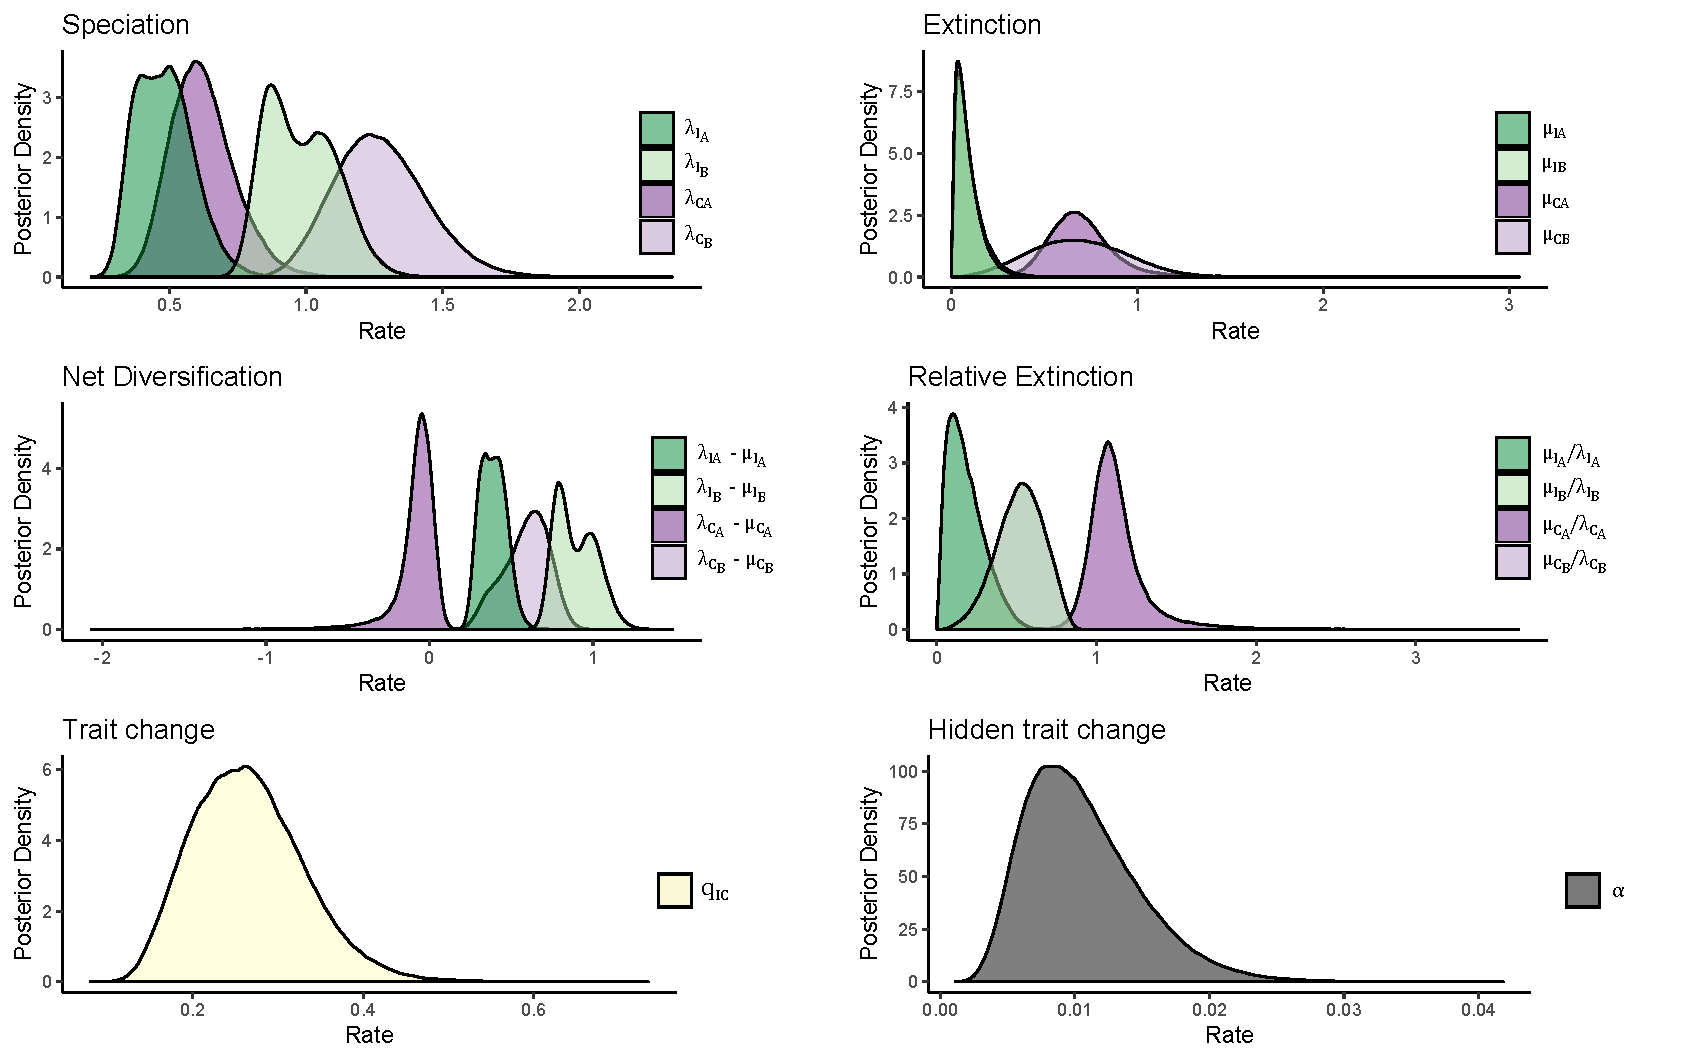
\includegraphics[width=\textwidth]{hisseSInoretposteriordist.pdf}
\caption{Posterior distribution for each of the parameters in the I/C-A/B breeding system model} % XXX
\label{suppfigure:ICAB}
\end{suppfigure}

\begin{suppfigure}
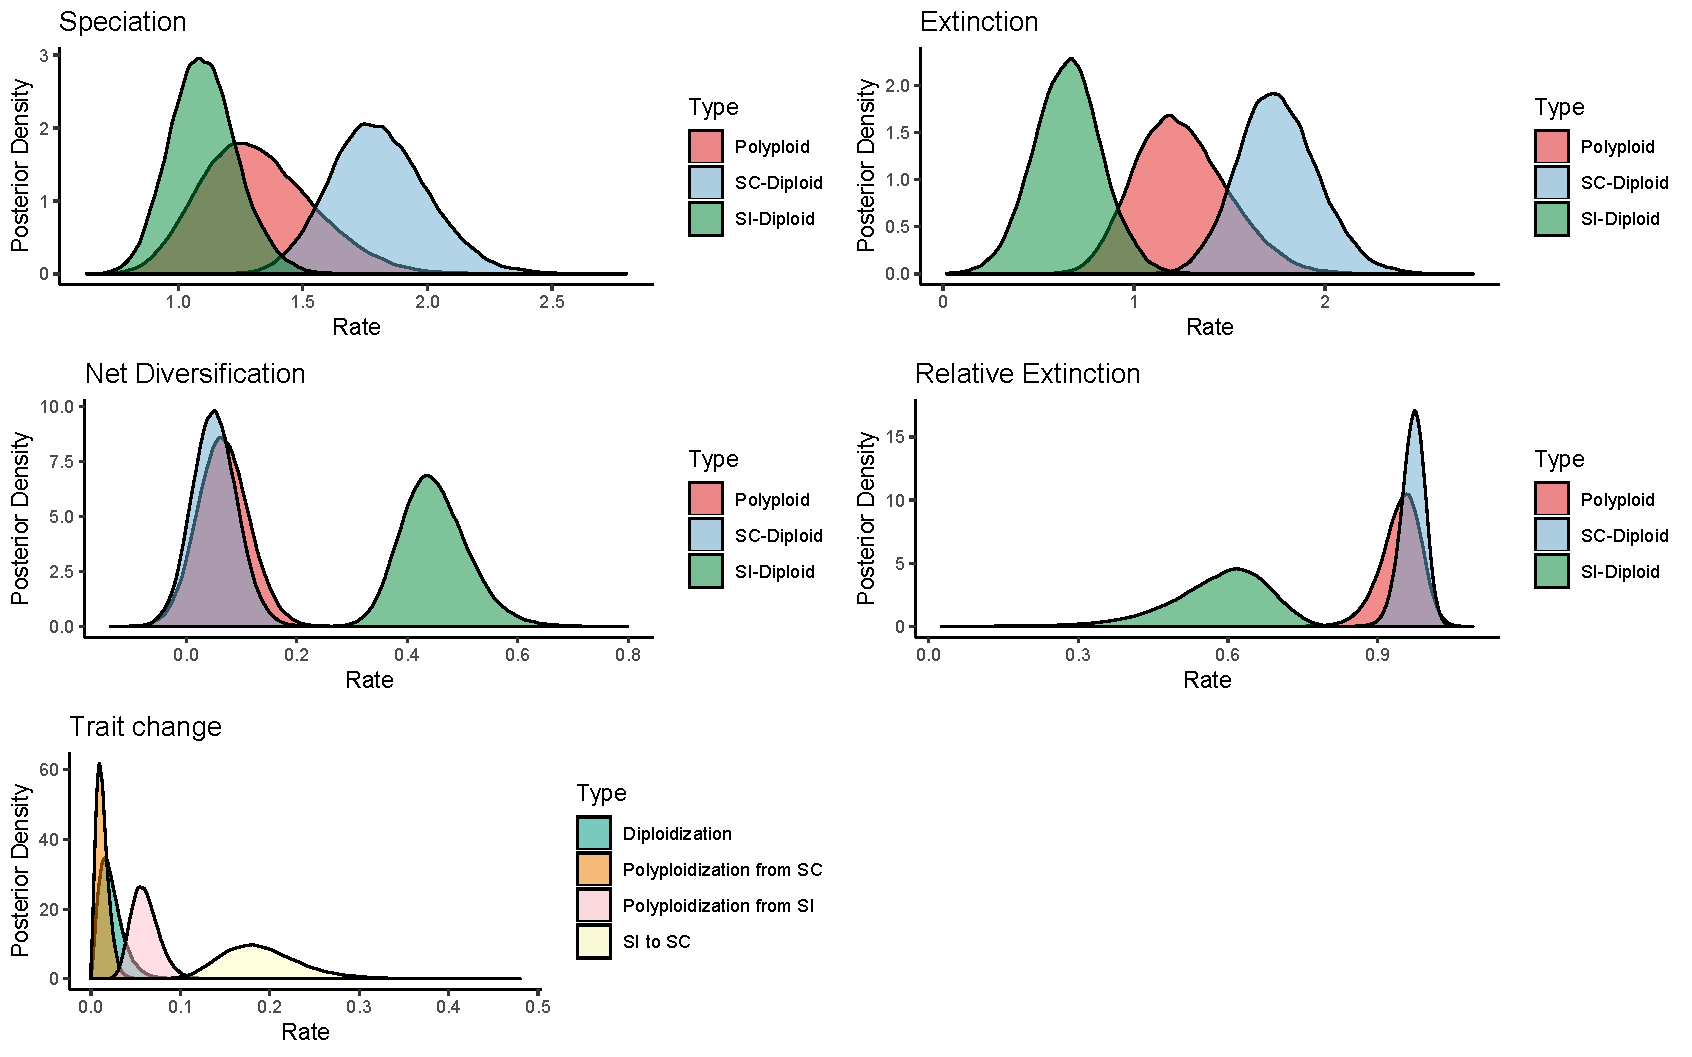
\includegraphics[width=\textwidth]{musseDPSIposteriordist.pdf}
\caption{Posterior distribution for each of the parameters in the ID/CD/CP polyploidy and breeding system model} % XXX
\label{suppfigure:IDCDCP}
\end{suppfigure}

\begin{suppfigure}
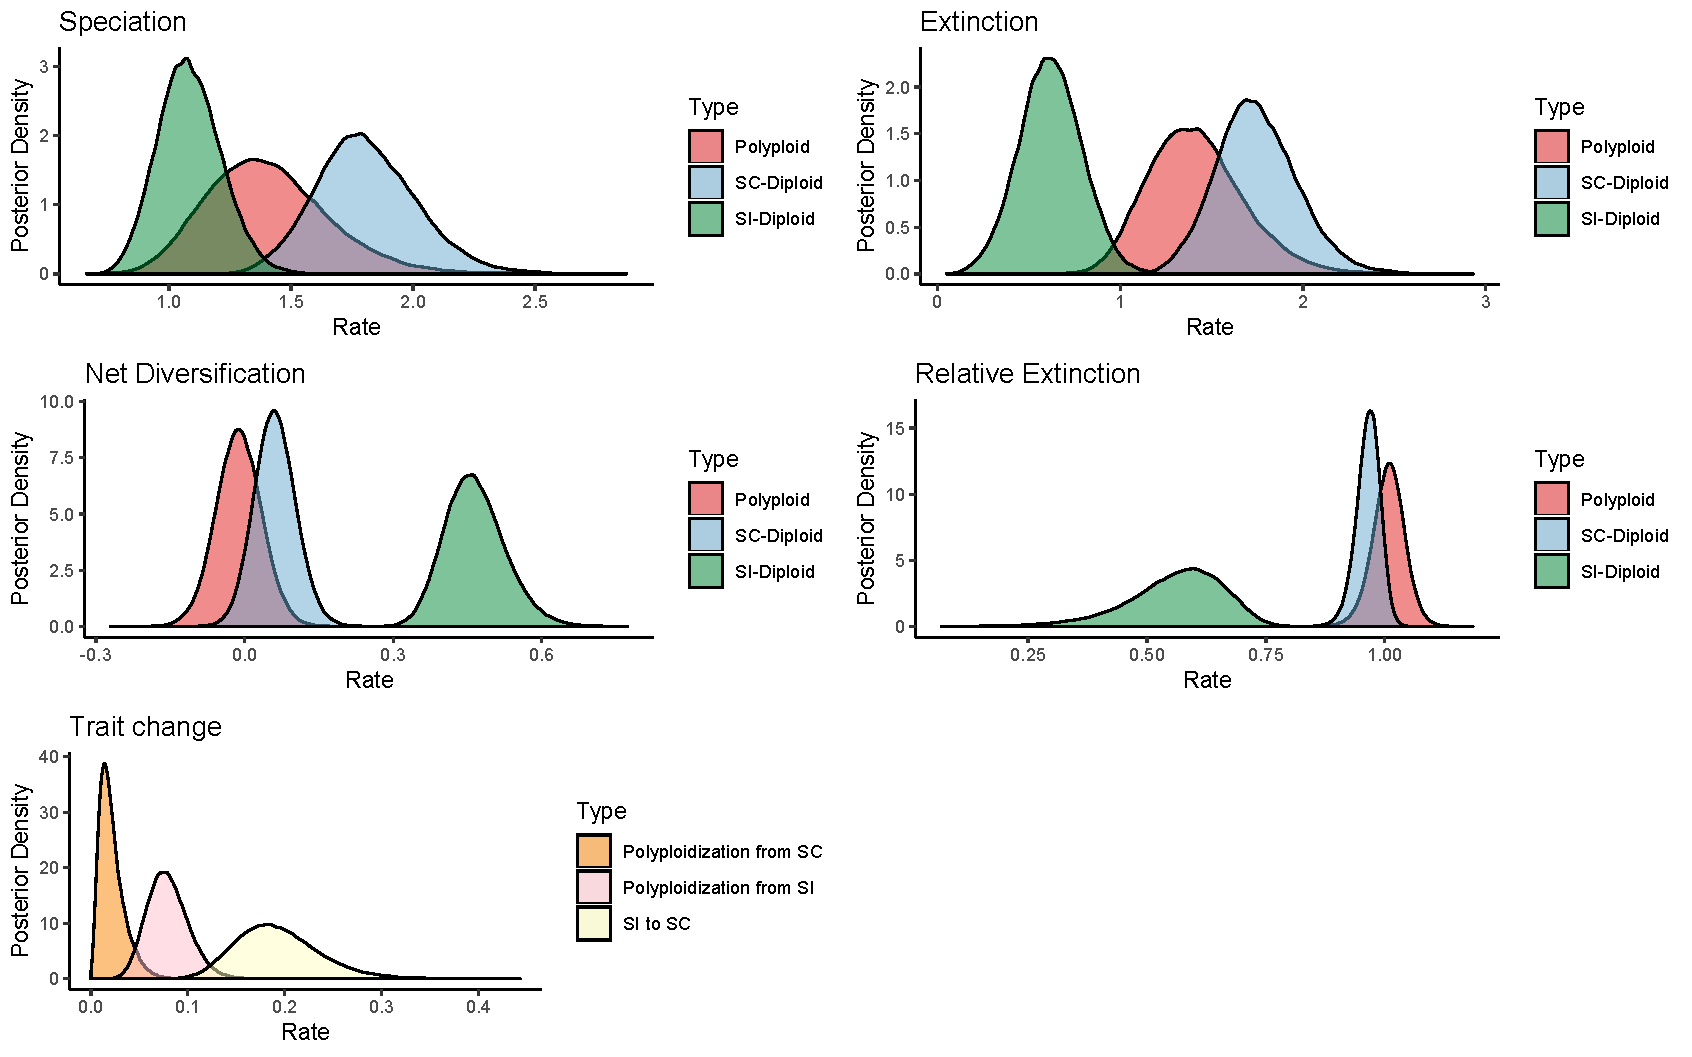
\includegraphics[width=\textwidth]{musseDPSInodipposteriordist.pdf}
\caption{Posterior distribution for each of the parameters in the ID/CD/CP no $\delta$ polyploidy and breeding system model} % XXX
\label{suppfigure:IDCDCPnodip}
\end{suppfigure}

\begin{suppfigure}
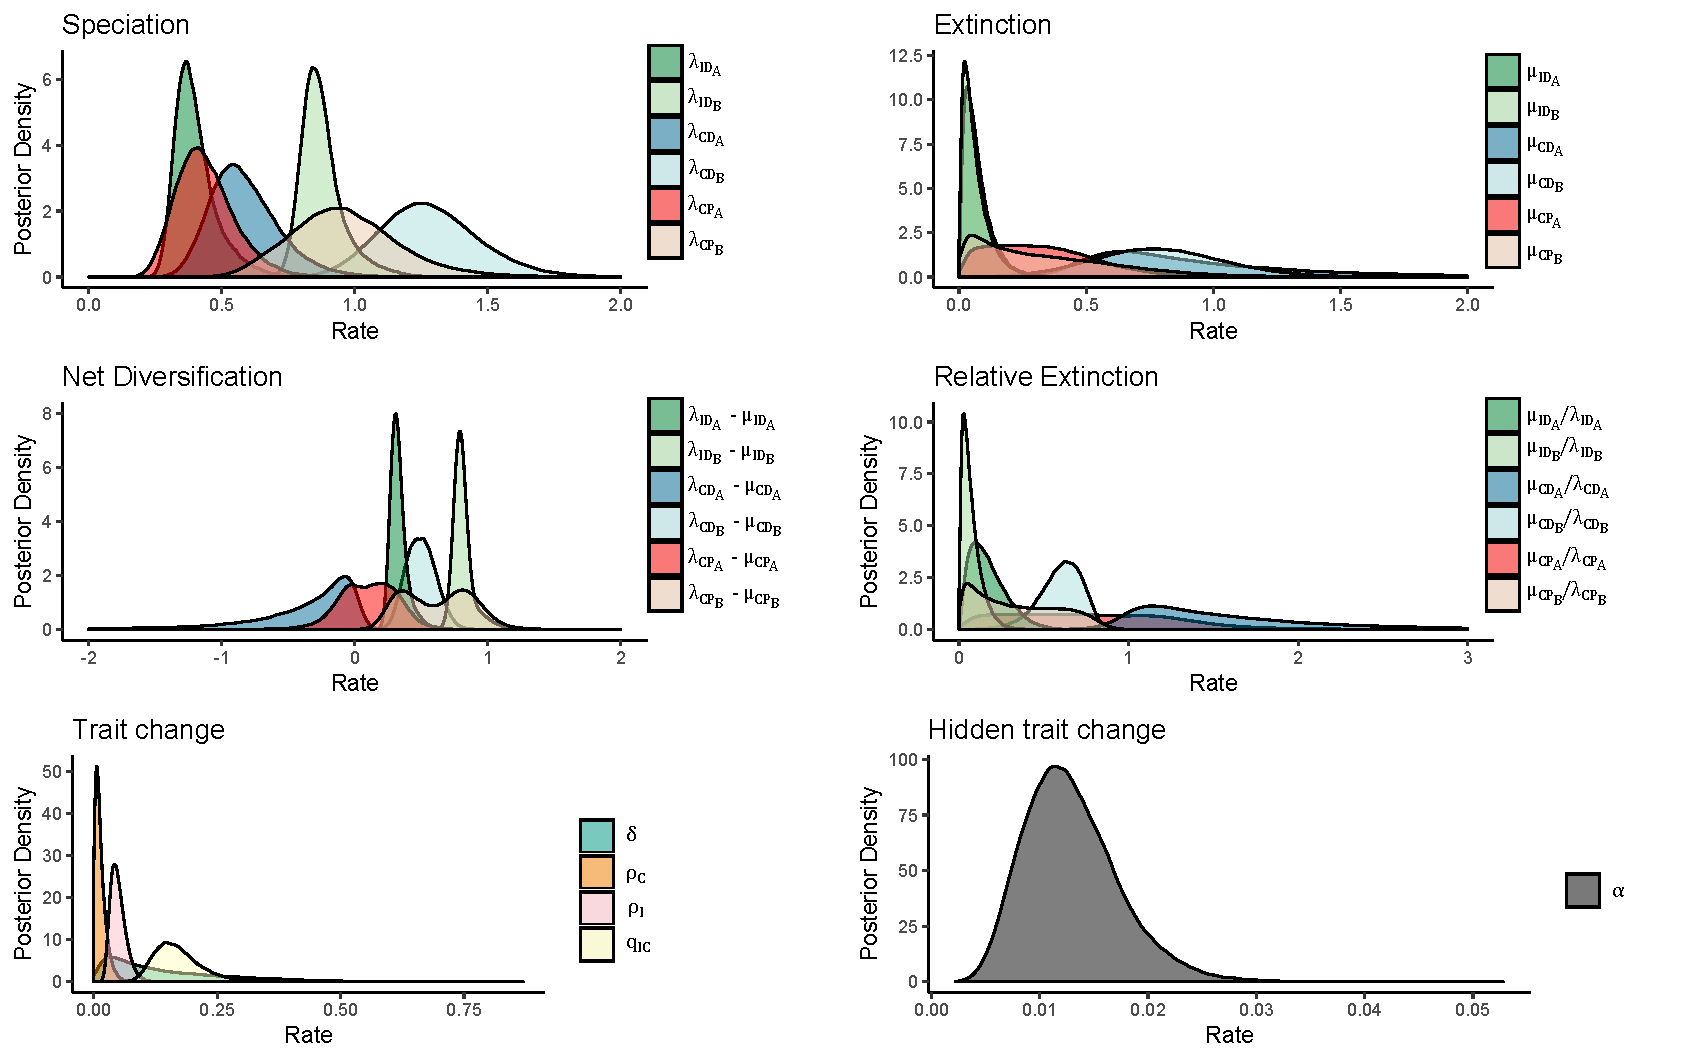
\includegraphics[width=\textwidth]{muhisseDPSIposteriordist.pdf}
\caption{Posterior distribution for each of the parameters in the ID/CD/CP-A/B polyploidy and breeding system model} % XXX
\label{suppfigure:IDCDCPAB}
\end{suppfigure}

\begin{suppfigure}
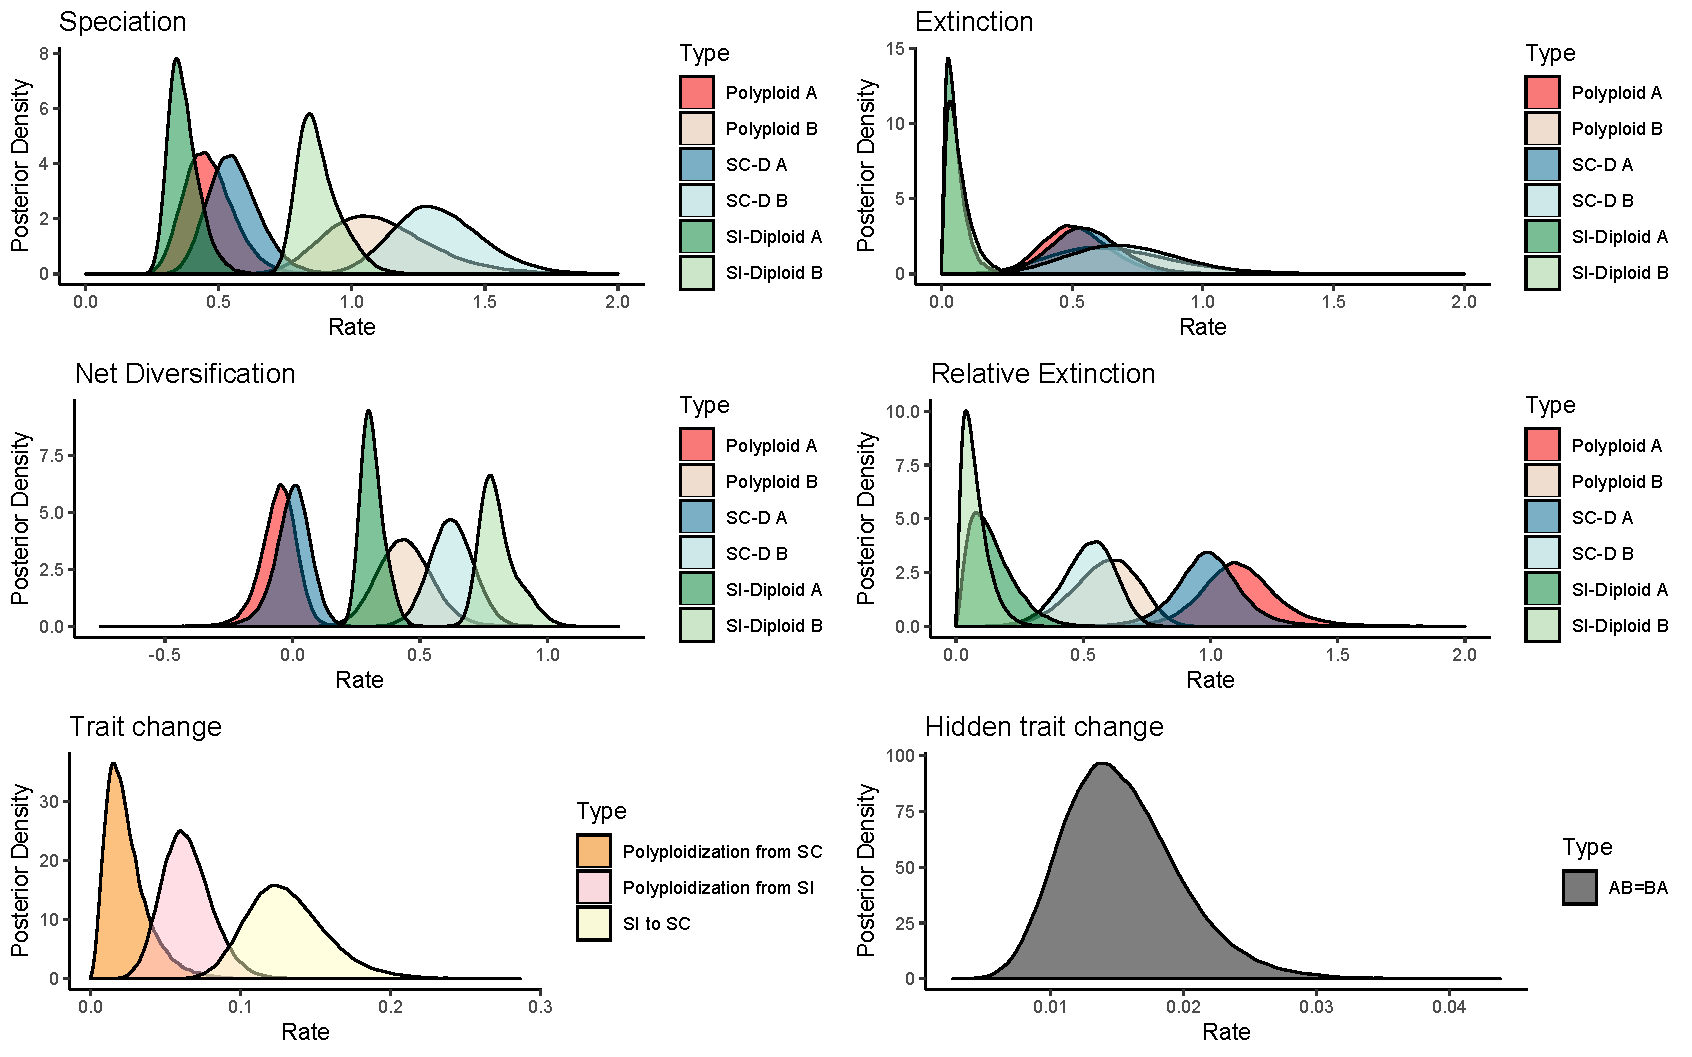
\includegraphics[width=\textwidth]{muhisseDPSInodipposteriordist.pdf}
\caption{Posterior distribution for each of the parameters in the ID/CD/CP no $\delta$- A/B polyploidy and breeding system model} % XXX
\label{suppfigure:IDCDCPnodipAB}
\end{suppfigure}
